\documentclass[11pt,a4paper]{article}
\usepackage[margin=2.5cm]{geometry}
\usepackage{amsmath,amssymb,bm,graphicx,booktabs}
\usepackage[colorlinks=true,linkcolor=blue,citecolor=blue]{hyperref}
\usepackage{enumitem}

\newcommand{\Pir}[1]{\Pi^{(\mathrm r)}_{#1}}
\newcommand{\Pis}[1]{\Pi^{(\mathrm s)}_{#1}}
\newcommand{\kt}{k_t}
\newcommand{\kperp}{\kappa_\perp}
\newcommand{\Ske}{Sk/\varepsilon}

\title{\vspace{-1.2em}Section 5 after the reconstruction:\\
what the results establish, and the revised claims}
\author{Sparsh Sharma (DLR Braunschweig)\\[0.2em]
\normalsize Results note for the revision of JFM-2026-1781 --- \today}
\date{}

\begin{document}
\maketitle
\vspace{-2em}

\paragraph{Summary.} Section~5 of the rejected manuscript --- the closure
of the rapid pressure--strain term on a single line --- was singled out by
two referees as the strongest part and by the third as not closed. Since
the rejection the section has been rebuilt on measured ground: (1) an
estimator that states exactly what line-of-sight data determine about the
rapid term and bounds it; (2) null tests on real and ODT turbulence that
validate the estimator and removed a 1\% initial-condition artifact from
the ODT runs; (3) a $128^3$ strained-box DNS with an exact-RDT companion
that measures the closure assumption A1 directly, as a function of
accumulated strain, and its control experiment showing the closure is
exact for axisymmetric distortion and that its plane-strain error is a
geometry property; (4) the correct linear reference for the projected
spectrum, which is \emph{not} the rigid translation the manuscript used;
(5) the verdict on ODT's slow-term allocation. This note collects the
numbers, states what Section~5 can now claim, lists the corrections the
manuscript needs, and names what is still open. Companion notes: LOS
estimator (25~Aug), null tests (25~Aug), allocation derivation (26~Aug)
and allocation results (3~Sep).

\section{What the referees objected to, and which result answers it}

\begin{center}\small
\begin{tabular}{p{0.06\textwidth}p{0.50\textwidth}p{0.38\textwidth}}
\toprule
Ref. & objection & answered by \\
\midrule
3.2 & the closure is not closed: eqs.\ (5.7)--(5.10) still need
      $a(\kappa_2,\kperp)$, $c(\kappa_2,\kperp)$ and a $\kperp$ integration &
      \S\ref{sec:los}: the null space is stated exactly and the rapid
      term is bounded sharply; \S\ref{sec:dns}: the bound width is measured
      under real strain \\
1.2 & the original formulation was not used in any reported calculation &
      \S\ref{sec:dns}: the collapsed form and its A1 error are now
      evaluated on DNS spectra; the moment closure's reduction is verified \\
1.3 & the rapid closure orders the components wrongly under plane strain
      (spanwise overtakes upwash) & \S\ref{sec:order}: measured in the
      exact $\Pir{}$; localized in the LRR $b$-term, not in ODT \\
3.1 & the ``rigid translation'' linear-RDT benchmark is not derived and is
      wrong for the projected spectrum & \S\ref{sec:rdt}: it is wrong; the
      exact projected-RDT companion replaces it \\
1.1, 2 & model-versus-itself validation, no spectral benchmark &
      \S\ref{sec:dns}, \S\ref{sec:rdt}: the DNS and its RDT companion are
      the benchmark; the three-way comparison is the next figure \\
3.3 & A1 undefined, (5.8)--(5.10) underived & LOS note \S2 derives the
      forward map and the kernels from the two-scalar representation \\
\bottomrule
\end{tabular}
\end{center}

\section{What a line determines: the estimator}\label{sec:los}

Under A1 (axisymmetry about the line, mirror-symmetric, helicity-free) the
solenoidal spectrum tensor is $\Phi_{mn}=a\,P_{mn}+c\,\xi_m\xi_n$ with two
scalars $(a,c)(\kappa_2,\kperp)$, realizable iff $a\ge0$, $a+(1-x)c\ge0$,
$x=\kappa_2^2/\kappa^2$. The line carries $\phi_{11}=\phi_{33}$ and
$\phi_{22}$ --- two weighted $\kperp$-integrals per $\kappa_2$ of two
unknown functions of $\kperp$: the null space is infinite-dimensional, and
this is Referee~3.2 stated exactly. But the target $\Pir{nn}$ is linear in
$(a,c)$ with the manuscript's kernels $g_n(x)$, so its extreme values over
everything consistent with the line data and realizability are a family of
linear programs, one per $\kappa_2$, giving sharp bounds
$[\Pi^-_{nn},\Pi^+_{nn}]$ and the kinematic indeterminacy
$\mathcal I_n=(\Pi^+-\Pi^-)/2\kt S$. Isotropic calibration (von K\'arm\'an
spectrum; 21-test suite pinning tracelessness, the angular averages
$+\tfrac15:-\tfrac15:0$, the longitudinal--transverse relation and the
exact $\tfrac45\kt S_{ij}$):
\begin{center}\small
\begin{tabular}{lccc}
\toprule
constraint level & $\mathcal I_{11}$ & $\mathcal I_{22}$ & $\mathcal I_{33}$\\
\midrule
line data $+$ solenoidality $+$ realizability (raw) & 0.77 & 1.28 & 0.86\\
$+$ log-Lipschitz slope cap $\lambda=4$ & $<5\%$ narrower & & \\
$+$ polarization cap $|c|\le\gamma a$, $\gamma=0$ & 0.34 & 0.58 & 0.24\\
$+$ both & 0.29 & 0.50 & 0.21\\
\bottomrule
\end{tabular}
\end{center}
Two free on-line falsifiers come with the forward map: (T1)
$\phi_{11}=\phi_{33}$ at every $\kappa_2$ and (T2) vanishing cross
spectra; any measured transverse splitting is a wavenumber-resolved
violation of A1 that the line itself reports.

\emph{Claim for \S5:} the rapid term is determined by line data up to a
quantified interval; A1 is not assumed but measured (T1) and, where it
fails, its effect on $\Pir{}$ is bounded. Smoothness does not narrow the
interval; polarization does --- and \S\ref{sec:dns} shows polarization is
$O(1)$ under strain, so the honest bound in the strained regime is the raw
one.

\section{Null tests}\label{sec:null}

JHTDB isotropic $1024^3$, 128 lines: T1 exceeds $2\sigma$ in 7\% of bins
(5\% by chance), T2 coherences $\sim0.01$, the derivative relation holds to
4\%, and the bounds bracket the Crow value at every constraint level; the
$b_{ij}$ noise floor is $\pm0.06$ at 128 lines. ODT nominal HIT (strain
machinery on, $A=0$, 1024 realizations): bounds bracket Crow at all times,
spectral nulls clean, and the pipeline found a real $b_{33}=+0.0148\pm0.0046$
bias, attributed by a reversal experiment to the ordered-Cholesky IC
whitening and removed by the symmetric $C^{-1/2}$ (all $|b_{ii}|\le0.005$
afterwards, T1 exceedances 0\%). Bookkeeping: the published runs carry the
1\% IC bias, far below the strain signal; all new runs use the fixed
initializer.

\section{The strained DNS: A1 measured, and the control}\label{sec:dns}

Pseudo-spectral $128^3$ box in a Rogallo deforming frame, decaying
precursor, plane strain $A=S\,\mathrm{diag}(\tfrac12,-\tfrac12,0)$ with
$\Ske\in\{0.8,16\}$ at onset, $e\le1$, 4 seeds, $\nu=10^{-2}$
($\kappa_{\max}\eta\approx0.76$ at $e=1$: a pilot resolution). Each run has
an exact-RDT companion (the same initial field evolved under the
closed-form Cauchy solution and projected identically). From the full
field: the exact $\Pir{ij}=A_{kl}M_{ijkl}$ by direct integration --- with
the Poisson factor~2 that the manuscript's displayed eq.\ (5.3) omits
(erratum) --- the exact azimuthal average, hence the true $(a,c)$ and the
discarded $m=2$ residue of $\Phi_{22}$ (the direct A1-violation measure),
the effective polarization $\gamma_{\rm eff}=|c|/a$, and the LOS bounds.

\begin{table}[h!]\centering\small
\begin{tabular}{c|ccccc|ccccc}
\toprule
& \multicolumn{5}{c|}{$\Ske=0.8$} & \multicolumn{5}{c}{$\Ske=16$}\\
$e$ & $b_{22}$ & $b_{22}^{\rm RDT}$ & $\gamma_{\rm eff}$ & $m{=}2$ & $\tfrac{\phi_{11}}{\phi_{33}}{-}1$
    & $b_{22}$ & $b_{22}^{\rm RDT}$ & $\gamma_{\rm eff}$ & $m{=}2$ & $\tfrac{\phi_{11}}{\phi_{33}}{-}1$\\
\midrule
0    & 0.003 & 0.003 & 0.10 & 0.133 & $+0.06$ & 0.003 & 0.003 & 0.10 & 0.133 & $+0.06$\\
0.25 & 0.036 & 0.038 & 0.50 & 0.162 & $-0.10$ & 0.038 & 0.038 & 0.52 & 0.185 & $-0.07$\\
0.5  & 0.064 & 0.071 & 0.79 & 0.166 & $-0.20$ & 0.070 & 0.071 & 1.28 & 0.247 & $-0.21$\\
0.75 & 0.091 & 0.099 & 1.09 & 0.172 & $-0.26$ & 0.099 & 0.099 & 2.42 & 0.318 & $-0.34$\\
1    & 0.125 & 0.123 & 1.44 & 0.189 & $-0.32$ & 0.124 & 0.123 & 4.22 & 0.396 & $-0.46$\\
\bottomrule
\end{tabular}
\caption{Plane strain: upwash anisotropy against its RDT companion,
effective polarization, A1-violation residue (isotropic floor 0.133) and
the on-line falsifier T1.}
\label{tab:dns}
\end{table}

\begin{table}[h!]\centering\small
\begin{tabular}{cc|ccc|cc}
\toprule
$\Ske$ & $e$ & exact $\Pir{11}$ & $\Pir{22}$ & $\Pir{33}$ & raw bound brackets? & $\gamma{=}0$ brackets?\\
\midrule
0.8 & 0.25 & 0.37 & $-0.43$ & 0.06 & yes & no\\
0.8 & 0.5  & 0.36 & $-0.45$ & 0.09 & no ($\Pir{11}$ 4\% out) & no\\
0.8 & 1    & 0.31 & $-0.45$ & 0.14 & no (37\% out) & no\\
16  & 0.25 & 0.35 & $-0.42$ & 0.08 & yes & no\\
16  & 0.5  & 0.31 & $-0.46$ & 0.15 & yes & no\\
16  & 1    & 0.23 & $-0.50$ & 0.27 & no & no\\
\bottomrule
\end{tabular}
\caption{Exact rapid term (per $\kt S$) and whether the LOS bounds contain
it. The raw kinematic bound is valid to $e\approx0.25$--$0.5$; the
polarization-capped bound never is under strain, because
$\gamma_{\rm eff}$ reaches $O(1)$ by $e=0.5$.}
\label{tab:bounds}
\end{table}

\paragraph{Reading.} (i) The A1 error is not $O(b^2)$-small: the residue
grows from its isotropic floor to $0.19$ ($\Ske=0.8$) and $0.40$
($\Ske=16$) by $e=1$, larger at rapid strain because eddies restore
axisymmetry at moderate $\Ske$. (ii) The raw bound brackets the exact term
early and fails as A1 fails --- the failure is A1's, not the estimator's.
(iii) The $\gamma=0$ cap, which does the narrowing in the isotropic
calibration, is illegitimate under strain. (iv) $b_{22}(e)$ follows RDT at
both ratios: the upwash amplification the leading-edge problem consumes is
linear to $e=1$.

\paragraph{The control (Fig.~\ref{fig:a1}).} Same box, axisymmetric
contraction $A=S\,\mathrm{diag}(\tfrac14,-\tfrac12,\tfrac14)$ (matched
$A_{22}$; A1 exact by symmetry) against plane strain at $\Ske=16$: the
residue stays at the floor ($0.133\to0.129$) and the splitting at zero
($+0.06\to0.00$) at every $e$, while under plane strain they grow to
$0.40$ and $-0.46$; $b_{22}(e)$ is identical in the two geometries
($0.124$ vs $0.117$ at $e=1$; $0.125$ vs $0.126$ at $\Ske=0.8$).
\emph{The single-line closure is exact for axisymmetric distortion, its
plane-strain error is a strain-geometry property that is now quantified,
and the acoustically relevant quantity is geometry-robust.} For the
application: a rounded/three-dimensional nose is an axisymmetric
stagnation strain (closure exact); a two-dimensional leading edge is plane
strain (closure needs the measured correction).

\begin{figure}[h!]\centering
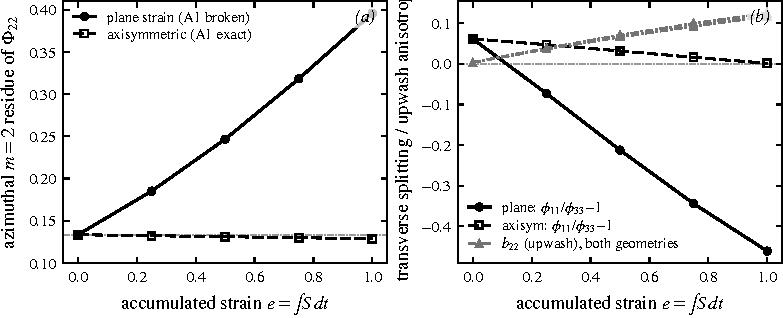
\includegraphics[width=\textwidth]{../post/closure_bound/strained/fig_a1_control.pdf}
\caption{A1 control at $\Ske=16$, $128^3$, 4 seeds. Left: azimuthal $m=2$
residue of $\Phi_{22}$. Right: transverse splitting and $b_{22}$.}
\label{fig:a1}
\end{figure}

\section{The correct linear reference: RDT does not translate the line
spectrum rigidly}\label{sec:rdt}

The manuscript's \S4.2.1 takes the eddy-free, inviscid ODT run as ``the
linear rapid-distortion result'': a rigid translation
$\kappa_2\to\kappa_2e^{e/2}$ of the component spectra without change of
shape. Referee~3.1 objected that the amplitude of each mode depends on
its full three-dimensional wavevector, so the projected spectrum cannot
translate rigidly. The exact-RDT companions settle it
(Fig.~\ref{fig:rdt}, left). Define the shape ratio
$R_{nn}(\kappa_2)=[\phi_{nn}(\kappa_2,e)/\!\int\!\phi_{nn}]\,/\,
[\phi_{nn}(\kappa_2e^{-e/2},0)/\!\int\!\phi_{nn}]\,e^{-e/2}$, equal to~1
at every $\kappa_2$ iff the translation is rigid:
\begin{center}\small
\begin{tabular}{lcccccccc}
\toprule
$\kappa_2(e)/\kappa_c(0)$ & 0.5--0.75 & 0.75--1.2 & 1.2--1.9 & 1.9--3 & 3--4.8 & 4.8--7.6 & 7.6--12\\
\midrule
$R_{22}$ (upwash), $e=1$ & 1.60 & 0.99 & 0.75 & 0.61 & 0.51 & 0.44 & 0.38\\
$R_{11}$, $e=1$          & 1.27 & 1.10 & 0.97 & 0.88 & 0.81 & 0.78 & 0.75\\
$R_{33}$, $e=1$          & 0.92 & 1.11 & 1.00 & 0.96 & 0.92 & 0.90 & 0.88\\
\bottomrule
\end{tabular}
\end{center}
Exact linear RDT redistributes the projected upwash spectrum toward low
$\kappa_2$ by a factor four across the resolved range at $e=1$
(modes aligned with the line, $x\to1$, are amplified least). What the
manuscript's Fig.~4 shows is the kinematics of a uniformly dilated line
acted on by a wavenumber-independent operator --- a property of ODT, not
of RDT. \emph{Consequence for \S4.2 and the abstract:} the ``broadband
versus rigid'' distinction conflates the two; the departure from rigid
translation that the manuscript attributes to the eddy cascade is, in
exact linear theory, already present. The three-way comparison --- ODT,
exact projected RDT, DNS --- on the same bands is the figure that replaces
Figs.~4--10's narrative; the data for it (the $S=2$ ODT ensembles of the
allocation campaign, the companions, the DNS) are all in hand and it is
the first open item below.

\paragraph{The splitting's scale dependence is nonlinear
(Fig.~\ref{fig:rdt}, right).} Exact RDT deepens the transverse splitting
with $\kappa_2$ ($-0.27$ at the energy-containing scales to $-0.58$ at ten
times the centroid; integrated $-0.47$). The DNS at $\Ske=0.8$ does the
opposite: $-0.36\to+0.02$ (integrated $-0.32$). The nonlinear return acts
within one turnover and reverses the linear trend at the small scales.
This reorders the diagnosis of ODT's rigid splitting (\S\ref{sec:alloc}):
the rapid operator $B$, uniform in $\kappa$, misses the linear deepening;
the eddies miss the nonlinear return; the two omissions cancel in the
integral, which is why ODT's integrated splitting ($-0.33$) matches the
DNS ($-0.32$). The $\kappa$-dependence of the \emph{linear} part is
exactly what the spectral kernel $g_n(x)$ of \S5 carries and the moment
closure discards: exercising eq.\ (5.7) in place of the algebraic closure
--- which the manuscript deferred to future work --- is now motivated by a
measured deficit, not by completeness.

\begin{figure}[h!]\centering
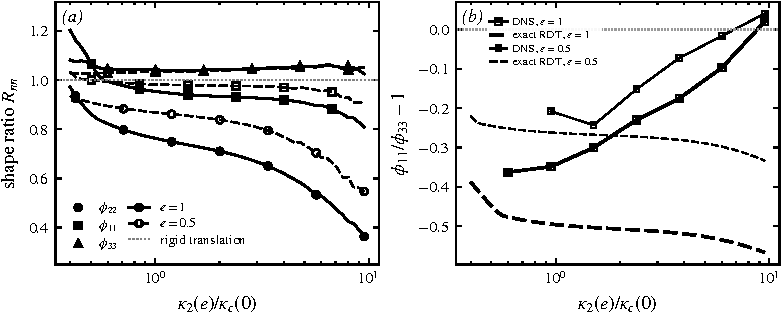
\includegraphics[width=\textwidth]{../post/closure_bound/strained/fig_rdt_projection.pdf}
\caption{Exact-RDT companions of the $128^3$ pilot, 4 seeds. Left: shape
ratio of the projected spectra to a rigid translation. Right: transverse
splitting versus wavenumber, exact RDT against DNS at $\Ske=0.8$.}
\label{fig:rdt}
\end{figure}

\section{Component ordering under plane strain}\label{sec:order}

Referee~1.3: the exact solution has the spanwise component overtaking the
upwash, both closures predict the opposite. Measured (Table~\ref{tab:bounds}):
at $e=1$ the exact $\Pir{33}/\kt S$ is $0.14$ at $\Ske=0.8$ and $0.27$ at
$\Ske=16$, exceeding $\Pir{11}$ ($0.23$) in the rapid case --- the
overtaking is real and sets in at rapid strain. LRR-QI gives
$\Pir{33}=0.58\,\kt S\,(b_{22}-b_{11})=0.143\,\kt S$ at $\Ske=0.8$
(matches) but half the value at $\Ske=16$; IP gives zero. The deficiency
lives in the $b$-dependent term of the moment closure. It is not an ODT
deficiency: the ODT moment-level $b_{ij}$ follows LRR to $\sim2\%$, and
$b_{33}$ stays within $0.006$ of zero at $e=1$ in every ODT run, against
the DNS $-0.010$. The spectral kernel with the $c$-scalar is where the
ordering is carried; the moment closure loses it.

\section{The slow term: allocation verdict}\label{sec:alloc}

The manuscript's no-double-counting argument (\S5.6) is now a measured
statement from both sides. Null test: ODT eddies generate no strain
signal at $A=0$. Rapid limit (allocation campaign, $\Ske=16$, under one
eddy per line in $e\le1$): every allocation rule --- isotropic kernel,
strain-biased \S6.2 generalization, eddy types --- reproduces exact RDT to
$\pm0.003$ in $b_{22}(e)$; the rapid term cannot be reached from inside the
eddy event, and the continuous operator carries it alone (the derivation
note shows the alternative overshoots $b_{22}(1)$ by $2.7\times$). At
$\Ske=0.8$ the eddies return $b_{22}$ by 10\% at $e=1$ and the rules differ
by $\le0.013$; the transverse splitting is rigid in $\kappa_2$ for every
rule (Fig.~\ref{fig:alloc}). Kernel energy allocation is not the lever for
the spectral distortion. Section~5's statement stands: rapid and slow
occupy disjoint terms by construction, and now by measurement.

\begin{figure}[h!]\centering
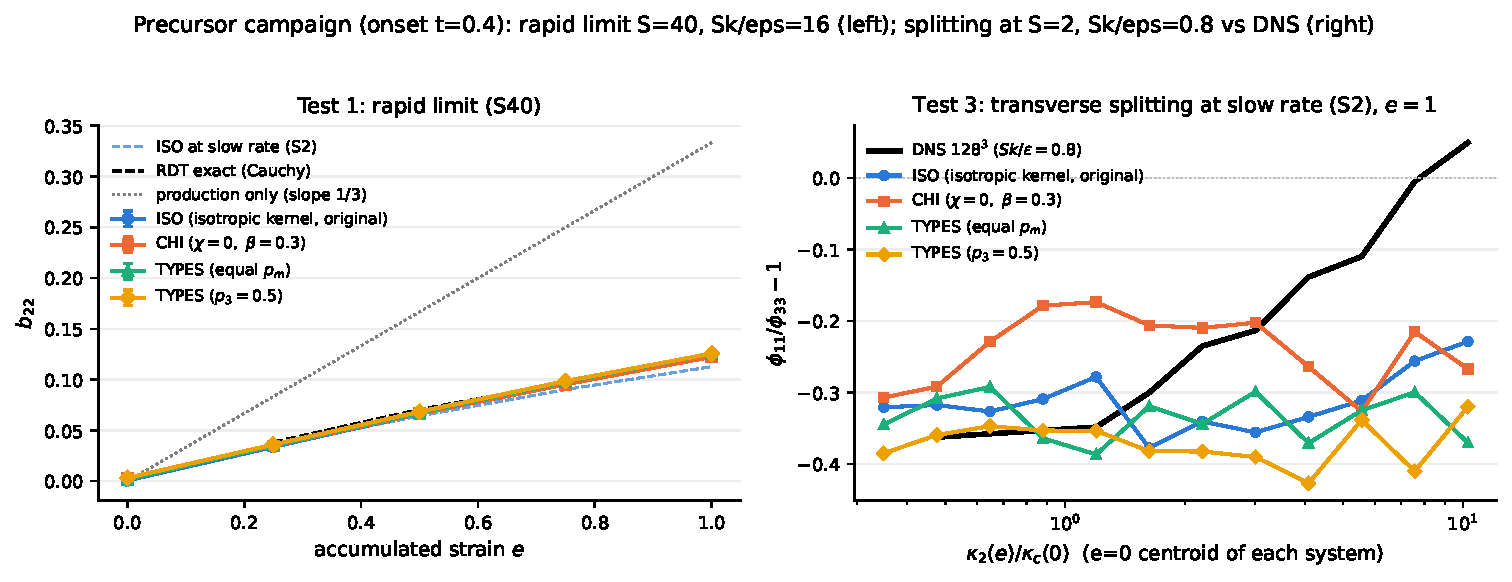
\includegraphics[width=\textwidth]{../post/closure_bound/odt_alloc/fig_alloc_tests_pre.pdf}
\caption{Allocation campaign ($8\times1024$ realizations, unstrained
precursor). Left: rapid limit, all rules on RDT. Right: splitting at
$\Ske=0.8$, every rule rigid against the DNS.}
\label{fig:alloc}
\end{figure}

\section{What Section 5 now claims}

\begin{enumerate}[leftmargin=2em,itemsep=2pt]
\item The rapid term is exactly $A_{kl}M_{ijkl}$ (with the factor~2);
  its single-line representation is obstructed by the azimuthal null
  space, stated exactly.
\item Under A1 it collapses to the kernel form; A1 is \emph{exact for
  axisymmetric distortion} and \emph{measured} under plane strain: the
  residue grows with $e$ and with $\Ske$ (Table~\ref{tab:dns}).
\item Independent of A1, line data bound the rapid term sharply; the
  bound is valid to $e\approx0.25$--$0.5$ under plane strain and is the
  honest statement of what the line closure delivers there.
\item The moment closure is the isotropic reduction of the kernel
  (verified); it reproduces $b_{ij}$ to $\sim2\%$ but discards the
  $\kappa$-dependence of the linear response and the component ordering
  at rapid strain, both now measured.
\item Rapid and slow terms are disjoint: verified by the $A=0$ null and
  by the rapid-limit test of every allocation rule.
\item The acoustically relevant quantity, $b_{22}(e)$, is linear to $e=1$
  and independent of strain geometry.
\end{enumerate}

\paragraph{Corrections to the manuscript.} (a) \S4.2.1: relabel the
eddy-free run as ODT kinematics; the linear reference is the exact
projected RDT, which is broadband (\S\ref{sec:rdt}). (b) Eq.\ (5.3):
Poisson factor~2. (c) Define A1 where it is first used (Ref.~3.3) and move
the derivation of the forward map and kernels (5.8)--(5.10) into an
appendix (LOS note \S2). (d) Replace the strain-on/strain-off figures by
the three-way comparison. (e) State the IC-whitening change. (f) Report
jackknife errors and realization counts throughout. (g) Cite the strained
DNS as the external benchmark (Ref.~1.1, 2) and Sagaut \& Cambon 2018
(Ref.~2).

\section{Open items}

\begin{enumerate}[leftmargin=2em,itemsep=2pt]
\item \emph{Three-way projected-spectrum comparison} at $\Ske=0.8$, $e\le1$:
  ODT ($S=2$ ensembles), exact RDT (companions), DNS, on common bands ---
  the replacement figure. Data in hand; half a day.
\item \emph{Resolution}: $128^3$ with $\kappa_{\max}\eta=0.76$ at $e=1$ is
  a pilot. A resolved run needs the restructured $256^3$ recipe (shared
  precursor checkpoint, seeds as a job array, $e\le0.5$); the pilot's
  conclusions are qualitative at the small scales.
\item \emph{Exercising eq.\ (5.7)} in the ODT rapid operator (a
  $\kappa$-dependent $B$ from the line spectra) --- the one change that
  can give ODT the linear $\kappa$-dependence; a scoping item, not a
  commitment.
\item \emph{ODT eddy population}: a forced or higher-$Re$ precursor to
  test whether small eddies supply the nonlinear return (allocation
  results note, item~1).
\item \emph{Leading-edge mapping} (Ref.~1.4): out of scope for \S5;
  belongs to the companion paper.
\item Code: the $S=40$ out-of-domain abort ($<1\%$ of realizations) in the
  line dilatation at very high strain rate.
\end{enumerate}

\end{document}
